
%(BEGIN_QUESTION)
% Copyright 2006, Tony R. Kuphaldt, released under the Creative Commons Attribution License (v 1.0)
% This means you may do almost anything with this work of mine, so long as you give me proper credit

Et av de mest grunnleggende forholdene i studiet av elektrisitet er {\it Ohms lov}.  Dette matematiske uttrykket relaterer flyten av elektrisk ladning ($I$, som vi kaller {\it strom}) til elektromotorisk potensial ($V$, som vi kaller {\it spenning}) og motstand mot ladningsflyt ($R$, som vi kaller {\it motstand}):

$$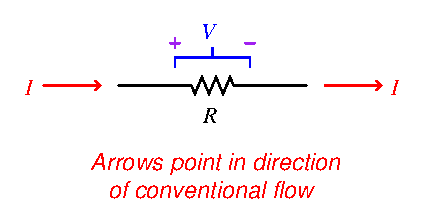
\includegraphics[width=15.5cm]{i00086x01.eps} I = {V \over R} \hbox{\hskip 10pt} \hbox{(For alle forhold)}$$

Forholdet mellom {\bf vaeske}-stromningsrate, trykkfall og ``motstand'' for en rorinnsnevring (orifice, strupeventil, rorbøy, osv.) er ikke like enkelt.  Ingen enkel matematisk formel er tilstrekkelig for a forutsi stromningsrater under alle forhold:

$$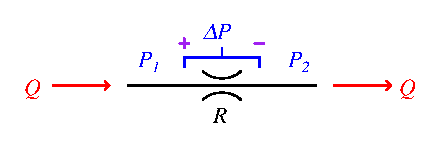
\includegraphics[width=15.5cm]{i00086x02.eps}$$

$$Q = {{P_1 - P_2} \over R_1} = {\Delta P \over R_1} \hbox{\hskip 10pt}  \hbox{(Kun for laminare stromningsforhold)}$$

\vskip 10pt

$$Q = \sqrt{{P_1 - P_2} \over R_2} = \sqrt{\Delta P \over R_2} \hbox{\hskip 10pt}  \hbox{(Kun for turbulente stromningsforhold)}$$

Shuntmotstander kan brukes som strommalende elementer, og produserer et spenningsfall i presis proporsjon med strommen gjennom dem.  Alt vi trenger a vite er shuntmotstanden, og vi kan inferere strom ved a male spenning.  Pa tilsvarende mate kan orificer brukes som vaeskestrommalende elementer, og produserer et trykkfall som varierer med mengden strom som passerer gjennom den:

$$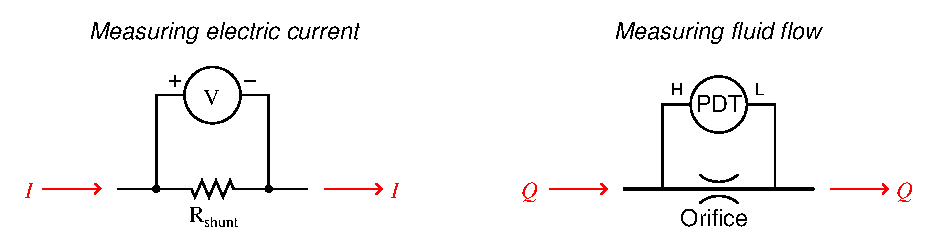
\includegraphics[width=15.5cm]{i00086x03.eps}$$

Gitt ``Ohms lov''-ligningene vist for vaeskestrom, identifiser hva vi ma vite for a bruke en orifice som en nøyaktig vaeskestrommalende enhet, og hvordan vi kan innhente denne informasjonen.  Identifiser ogsa typen malende instrument vi trenger for a male trykket, slik at vi kan beregne stromningsraten fra avlesningen.

\underbar{file i00086}
%(END_QUESTION)





%(BEGIN_ANSWER)

Her er det vi ikke vet om strommalingsscenarioet stromningsregimet (laminart eller turbulent), og ogsa hva ``motstanden'' til vaeskerestriksjonen er.  Selvfolgelig vil Reynolds-tallet for strommen indikere hvilket regime den er i, og $R$-faktoren for orificen kan enten bestemmes eksperimentelt eller utledes fra orifice-ligninger (tilgjengelig i enhver grundig referansebok).

\vskip 10pt

Det riktige trykkmalingsinstrumentet for vaeskestrom er et {\it differansetrykk}-instrument, slik som en DP-celle eller DP-manometer, eller kanskje til og med et kvikksolvmanometer.


%(END_ANSWER)





%(BEGIN_NOTES)

Hvis noen spors, bruker jeg indeks for a skille ``motstands''-verdiene $R_1$, $R_2$, osv. for a vise at ``motstands''-faktoren vil vaere forskjellig for hvert stromningsregime.

%INDEX% Physics, dynamic fluids: Resistance of liquid flow component

%(END_NOTES)


